\documentclass[12pt]{article}
\usepackage[top=1in, bottom=1in, left=1in, right=1in]{geometry}
%\usepackage[margin=1in]{geometry}
\usepackage[onehalfspacing]{setspace}
%\usepackage[doublespacing]{setspace}
\usepackage{amsmath, amssymb, amsthm}
\usepackage{enumerate, enumitem}
\usepackage{fancyhdr, graphicx, proof, comment, multicol}
\usepackage[none]{hyphenat} % This command prevents hyphenation of words
\binoppenalty=\maxdimen % This command and the next prevent in-line equation breaks
\relpenalty=\maxdimen
%    Good website with common symbols
% http://www.artofproblemsolving.com/wiki/index.php/LaTeX%3ASymbols
%    How to change enumeration using enumitem package
% http://tex.stackexchange.com/questions/129951/enumerate-tag-using-the-alphabet-instead-of-numbers
%    Quick post on headers
% http://timmurphy.org/2010/08/07/headers-and-footers-in-latex-using-fancyhdr/
%    Info on alignat
% http://tex.stackexchange.com/questions/229799/align-words-next-to-the-numbering
% http://tex.stackexchange.com/questions/43102/how-to-subtract-two-equations
%    Text align left-center-right
% http://tex.stackexchange.com/questions/55472/how-to-make-text-aligned-left-center-right-in-the-same-line
\usepackage{microtype} % Modifies spacing between letters and words
\usepackage{mathpazo} % Modifies font. Optional package.
\usepackage{mdframed} % Required for boxed problems.
\usepackage{parskip} % Left justifies new paragraphs.
\linespread{1.1} 


%figure support
\usepackage{import}
\usepackage{xifthen}
\pdfminorversion=7
\usepackage{pdfpages}
\usepackage{transparent}
\newcommand{\incfig}[1]{%
	\def\svgwidth{\columnwidth}
	\import{./figures/}{#1.pdf_tex}
}
\graphicspath{ {./figures/} }
\pdfsuppresswarningpagegroup=1

\newenvironment{problem}[1]
{\begin{mdframed}[linewidth=0.8pt]
        \textsc{Problem #1:}

}
    {\end{mdframed}}

\newenvironment{solution}
    {\textsc{Solution:}\\}
    {\newpage}% puts a new page after the solution
    
\newenvironment{statement}[1]
{\begin{mdframed}[linewidth=0.6pt]
        \textsc{Statement #1:}

}
    {\end{mdframed}}

%\newenvironment{prf}
 %   {\textsc{Proof:}\\}
 %   {\newpage}% puts a new page after the solution

\begin{document}
% This is the Header
% Make sure you update this information!!!!
\noindent
\textbf{CNT 3004C-01 Introduction to Computer Networks} \hfill \textbf{Brandon Thompson} \\
\normalsize Prof. Ding \hfill Due Date: 4/23/2020 \\

% This is where you name your homework
\begin{center}
\textbf{Final Project}
\end{center}
	\begin{problem}
		Consider a scenario in which Host A wants to simultaneously send packets to Hosts B and C. A is connected to B and C via a broadcast channel -- a packet sent by A is carried by the channel to both B and C. Suppose that the broadcast channel connecting A, B, and C can independently lose and corrupt packets (and so, for example, a packet sent from A might be correctly received by B, but not by C). Design a stop-and-wait-like error-control protocol for reliably transferring packets from A to B and C, such that A will not get new data from the upper layer until it knows that both B and C have correctly received the current packet. The FSM for B should be essentially the same as for C.
	\end{problem}
	\begin{solution}
		Figure \ref{fig:snd} is the sender FSM for host A. The process starts with a call from
		the above layer, it then sends the data to hosts A and B
		with the sequence number 0. If A receives a corrupt packet from either host B or C it will
		resend the missed packet to both hosts. If A receives an ACK from both B and C then it will
		wait for a call from the above layer and send the packet with sequence 1 to B and C.
		The cycle will repeat with sequence 1, on error resend packet to both hosts, on ACK from
		both wait for above layer and set seq to 0.
		Because A has to wait for the ACK from both hosts before it checks the above layer, A
		will not pull new data until both hosts have ACK'ed without error.
		
		\begin{figure}[ht!]
			\centering
			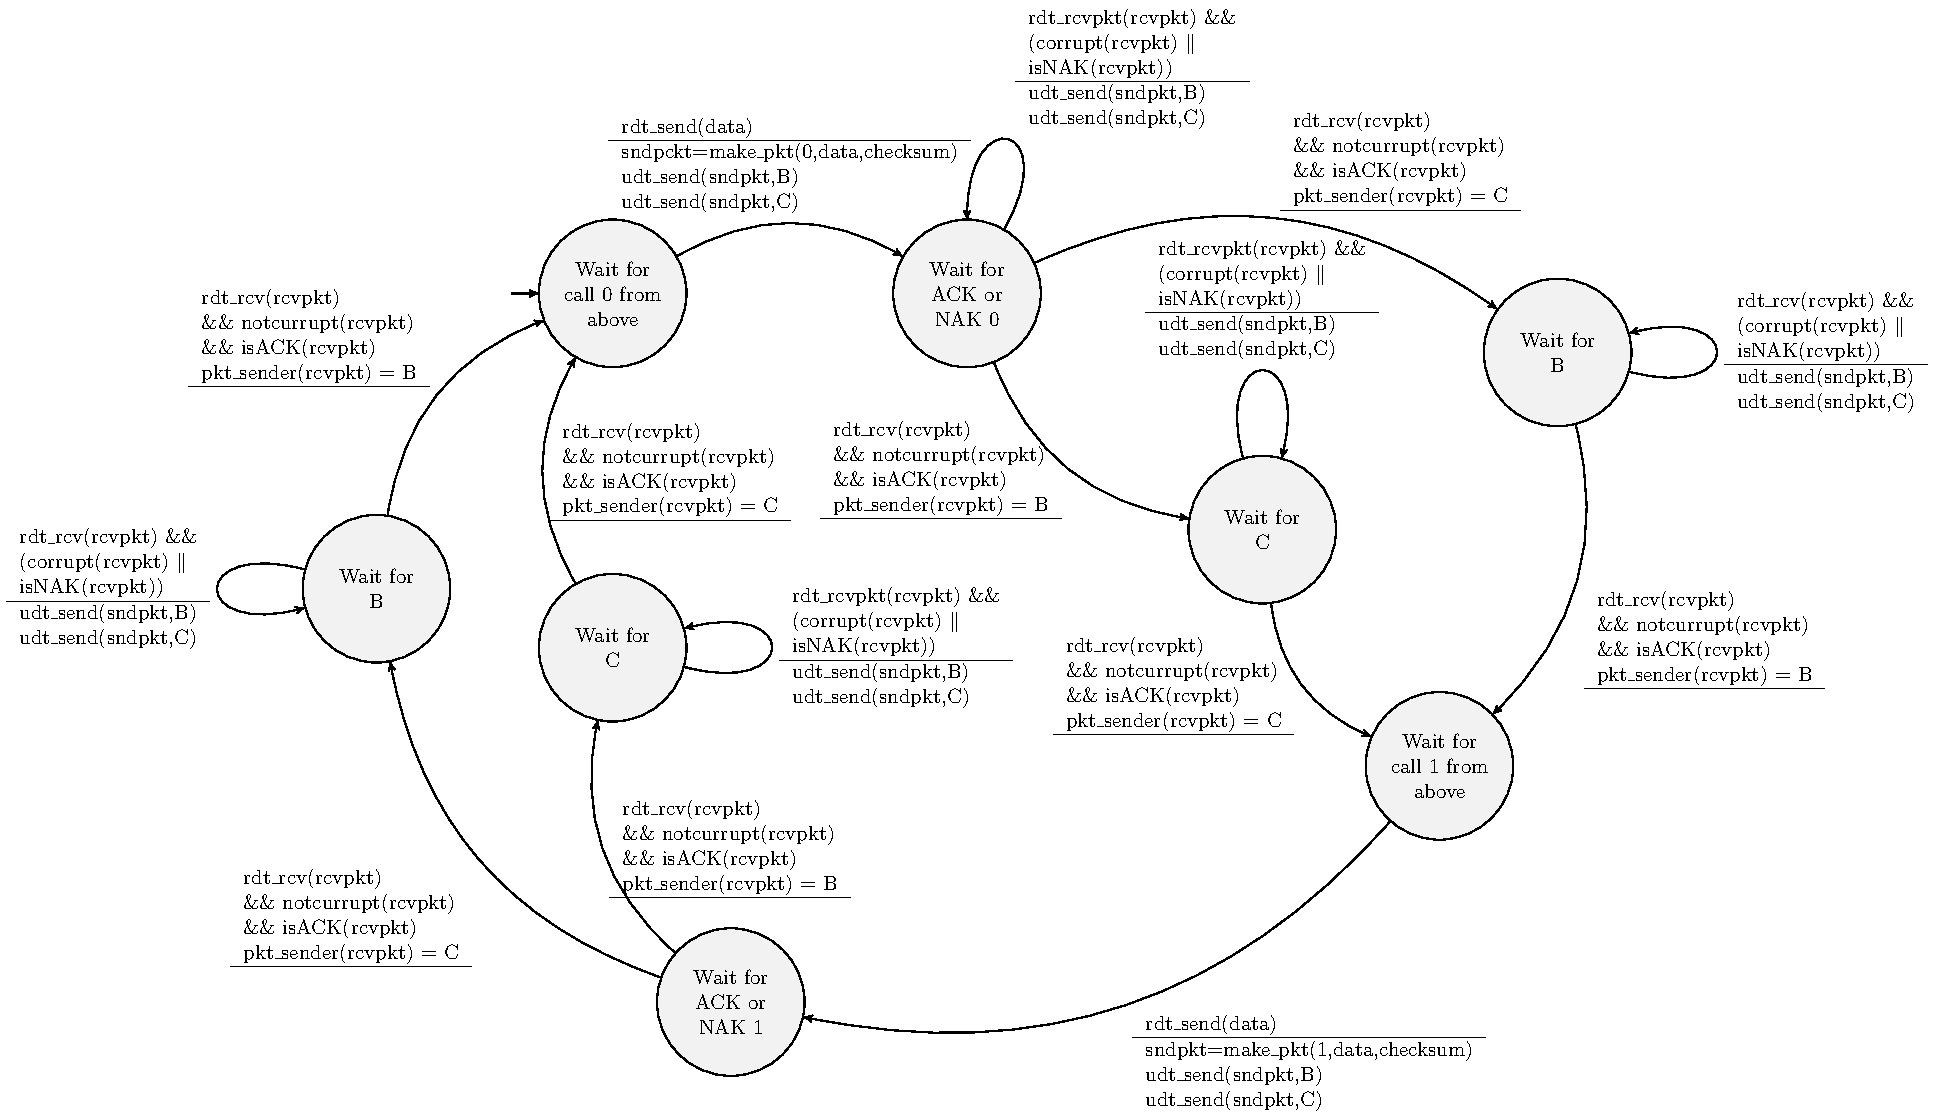
\includegraphics[width=\textwidth]{final_project_snd_fsm.pdf}
			\caption{Sender FSM for host A.}
			\label{fig:snd}
		\end{figure}

		Figure \ref{fig:rcv} shows the receiver FSM, hosts B and C will have similar FSM's 
		because they both behave the same way. Host B will wait for the packet with sequence 0
		from A, if the packet from A is corrupt, B will send a NAK to A, if the packet has a
		sequence number of 1, B will send an ACK and continue waiting for the sequence 0. If
		the packet sent by A is not corrupted and has a sequence of 0, B will extract and
		deliver the data and send an ACK to A, the n wait for a sequence 1 from A. The process
		repeats for sequence 1.

		\begin{figure}[ht!]
			\centering
			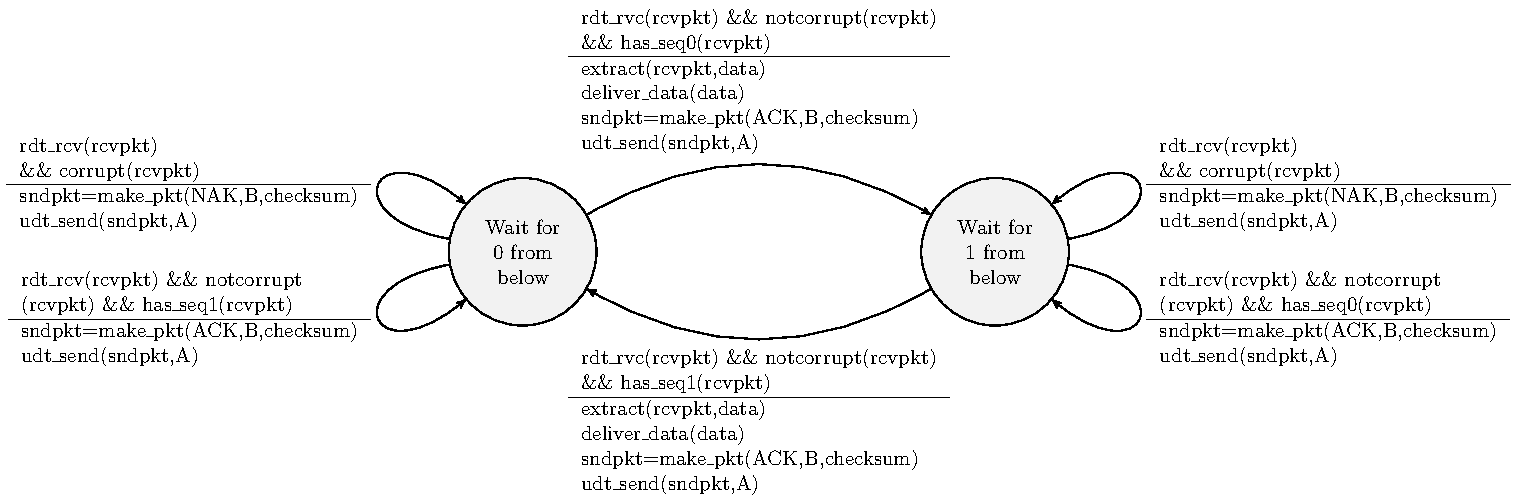
\includegraphics[width=\textwidth]{final_project_rcv_fsm.pdf}
			\caption{Receiver FSM for host B.}
			\label{fig:rcv}
		\end{figure}
		
		The packet format will include either a one or a zero for the sequence number, the sender of the packet, a data section (for data, ACK or NAK), and a checksum section.
	\end{solution}

\end{document}
